\documentclass[../main.tex]{subfiles}

\graphicspath{{\subfix{../imgs/}}}

\begin{document}

\section{Task 3.2}

Create a module (\textbf{ModuleDouble}) with two threads (A, B), one method (A) and four events (A, B, Aack, Back) as shown in Figure \ref{fig:moduledouble}. Thread A notifies event A every 3 ms and thread B notifies event B every 2 ms. After notification, the thread waits for an acknowledgement (event Aack and Back). If acknowledgement is not received after a timeout period (A = 3 ms and B = 2 ms), the threads continue notifying event A or B. The method A alternates between waiting on event A and B. Use dynamic sensitivity in the method by calling \textbf{next\_trigger()} to define the next event to trigger the method. Let the method print the current simulation time and the notified events.

\begin{figure}[h]
    \centering
    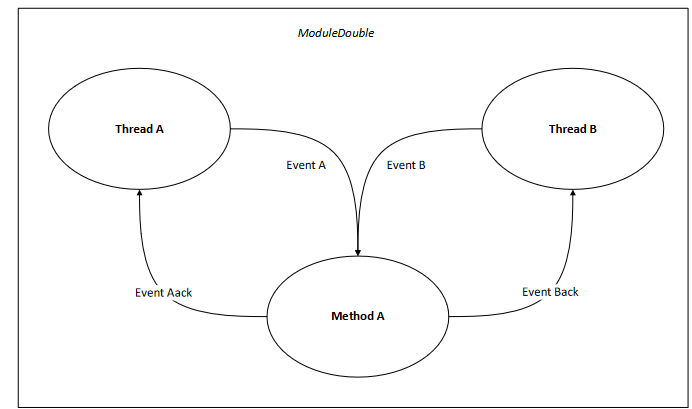
\includegraphics[width=0.9\textwidth]{task_3_2.png}
    \caption{ModuleDouble with method, threads and events.}
    \label{fig:moduledouble}
\end{figure}

\subsection*{Solution}

We start by defining a class \textbf{ModuleDouble}, inhereting from \textbf{sc\_module}, with the required methods and events.

\begin{myminted}{/inc/ModuleDouble.hpp}
class ModuleDouble : public sc_module {
public:
    /* Events */
    sc_event event_A, event_B, event_Aack, event_Back;

    ModuleDouble(sc_module_name name);
    ~ModuleDouble();

private:
    std::string moduleName;
    void thread_A();
    void thread_B();
    void method_A();
};
\end{myminted}

\newpage

Both \texttt{thread\_A} and \texttt{thread\_B} are functionally identical, with exception of which event they notify and the wait time. The implementation of \texttt{thread\_A} is seen below. After waiting the thread checks if \texttt{method\_A} acknowledged the event notify.

\begin{myminted}{/src/ModuleDouble.cpp (thread\_A)}
void ModuleDouble::thread_A() {
    while (true) {
        std::cout << "Thread A - Time: " << sc_time_stamp() << " - Notifying event_A\n";
        event_A.notify();

        wait(3, SC_MS);
        if (event_Aack.triggered()) {
            std::cout << "Thread A - Time: " << sc_time_stamp() << " - Received event_Aack\n";
        }
        else {
            std::cout << "Thread A - Time: " << sc_time_stamp() << " - Timeout on event_A\n";
        }
    }
}
\end{myminted}

To make \texttt{method\_A} switch between waiting on event A and B, we use dynamic sensitivity by calling \texttt{next\_trigger}. The full implementation of \texttt{method\_A} is seen below.

\begin{myminted}{/src/ModuleDouble.cpp (method\_A)}
void ModuleDouble::method_A() {
    if (event_A.triggered()) {
        std::cout << "Method A - Time: " << sc_time_stamp() << " - Handling event_A\n";
        event_Aack.notify();
        next_trigger(event_B);
    }
    else if (event_B.triggered()) {
        std::cout << "Method A - Time: " << sc_time_stamp() << " - Handling event_B\n";
        event_Back.notify();
        next_trigger(event_A);
    }
}
\end{myminted}

We set the simulation time to $20 \si{ms}$. The output from the first $10 \si{ms}$ of \textbf{ModuleDouble} is seen on the next page.

\newpage

\begin{mintedterminal}{a1\_32.exe}
Thread A - Time: 0 s - Notifying event_A
Thread B - Time: 0 s - Notifying event_B
Method A - Time: 0 s - Handling event_A
Thread B - Time: 2 ms - Timeout on event_B
Thread B - Time: 2 ms - Notifying event_B
Method A - Time: 2 ms - Handling event_B
Thread A - Time: 3 ms - Timeout on event_A
Thread A - Time: 3 ms - Notifying event_A
Method A - Time: 3 ms - Handling event_A
Thread B - Time: 4 ms - Timeout on event_B
Thread B - Time: 4 ms - Notifying event_B
Method A - Time: 4 ms - Handling event_B
Thread A - Time: 6 ms - Timeout on event_A
Thread A - Time: 6 ms - Notifying event_A
Thread B - Time: 6 ms - Timeout on event_B
Thread B - Time: 6 ms - Notifying event_B
Method A - Time: 6 ms - Handling event_A
Thread B - Time: 8 ms - Timeout on event_B
Thread B - Time: 8 ms - Notifying event_B
Method A - Time: 8 ms - Handling event_B
Thread A - Time: 9 ms - Timeout on event_A
Thread A - Time: 9 ms - Notifying event_A
Method A - Time: 9 ms - Handling event_A
Thread B - Time: 10 ms - Timeout on event_B
Thread B - Time: 10 ms - Notifying event_B
Method A - Time: 10 ms - Handling event_B
\end{mintedterminal}

\end{document}